\chapter{Future Work}
\label{chap:FutureWork}

In this chapter, we take up different possibilities and approaches to how the presented work around Shila can be improved and extended. The discussion refers to the results that are obtained in the course of this work and wants to provide the best possible basis for the further development of Shila.

\section*{Further testing}

After completion of the implementation, we checked and ensured the basic functionality of Shila in simple tests both in local and SCIONLab infrastructure. However, during the execution of the Shila Measurement, presented in the previous chapter, individual experiments occasionally failed. Of course, such experiments were repeated and not included in the measurements. The exact reasons for the failure have not been investigated in the course of this work, but the failed experiments have all been documented. An important part of the revision and further development of Shila is to use this documentation to identify and fix possible weaknesses and bugs. Hereby the infrastructure \cite{} developed for the execution of the measurements can be optimally used to perform further extensive test runs.

\section*{More flexible Routing-Information}

In the current version of Shila, there is only one way to pass the Routing-Information, i.e. the mapping from TCP Address to SCION Address. The information has to be passed along with the startup of the shim layer. This assumes that the mapping is already known and means a restriction in flexibility.  

One possible solution was investigated in the conceptual phase of the thesis: The record route option of the IP protocol allows to log the route of a datagram through the Internet. When enabled, each IP datagram has space in its header to store up to eight IP addresses that it encounters on its way from sender to receiver. A predefined data structure has to be specified during the creation of the socket to activate this optional socket option. This structure describes the 32 bytes of memory required for storing the addresses and can instead of the usual zero also be initialized with the SCION target address. Each packet sent from the socket created with this option contains the SCION destination address in its IP header. The SCION target address for a new Main-Flow can then be extracted by Shila from the first intercepted datagram. With a wrapper around the standard TCP API, the process of additional address specification can be made pleasant for the user. Of the 32 bytes of the record route option, 28 bytes can be used effectively. The first four bytes are overwritten when traversing the virtual interface on the way to Shila. A SCION address requires a maximum of 20 bytes. With this approach its therefore possible to pass further control information, up eight bytes, from the application to Shila. At first glance, this approach has the disadvantage of increasing the overhead. But there is nothing to be said against reassembling the IP packet in Shila without the additional option. The stated approach is not yet part of the implementation since not strictly needed for the basic functionality. But once part of Shila, it increases the flexibility and possibilities of the shim layer.

\section*{Reducing overhead}

As we have seen in the previous chapter, the data exchange with MPTCP over SCION comes with comparatively high overhead. This is also due to the multiple nesting of the payload within a SCION packet: It contains a Shila-Message\footnote{A Shila-Message is the message sent between two Shila instances via the Backbone-Connection.}, which itself holds a TCP segment in an IP datagram. The actual data sits inside the TCP packet. In this nesting, information is sent along which does not necessarily have to be transmitted. It is not necessary to include the source and destination address in the IP header, these are clearly defined by the TCP flow of the backbone connection. The same applies to the protocol identification number or the checksum, which can be recalculated. An approach to reduce overhead would, therefore, be to go without the IP header but just the TCP segment as payload and a custom header. Such a header holds only the information required to reassemble the IP packet at the receiving endpoint. An IP header without additional options has a size of 20 bytes. The identification value (2 bytes) and the flags together with the fragment offset (2 bytes) must be included in the custom header for every IP datagram processed by Shila. The remaining information necessary for the re-composition of the IP packet at the destination endpoint can either be calculated, e.g. the checksum, or is given through to the backbone connection, e.g. source and destination address. With this approach, the contribution of the IP header to overhead can be reduced by 80\%. Redundant information is also sent in the TCP segment, the source and destination ports are also given by the backbone connection. But the savings potential for combining the TCP header is lower, the majority of the fields contain dynamic information. If the proposal under discussion is implemented, the additional effort for parsing and recompiling the IP datagrams should not be disregarded.

\section*{Shorter distances with XDP}

Interposing Shila between MPTCP and SCION inevitably increases the round-trip time and has a negative effect on throughput. Besides the computational effort within the shim layer, using Shila means for the data an additional loop through the kernel networking functionality in both endpoints, as illustrated on the left side of Figure \ref{fig:ShilaDetourKernel}. Its therefore desirable to shorten this additional detour in future work and therefore the improve the performance of Shila. A possible technology that could be used for this improvement is XDP.

\begin{figure}[H]
	\begin{center}
		\def\svgwidth{1\textwidth}
		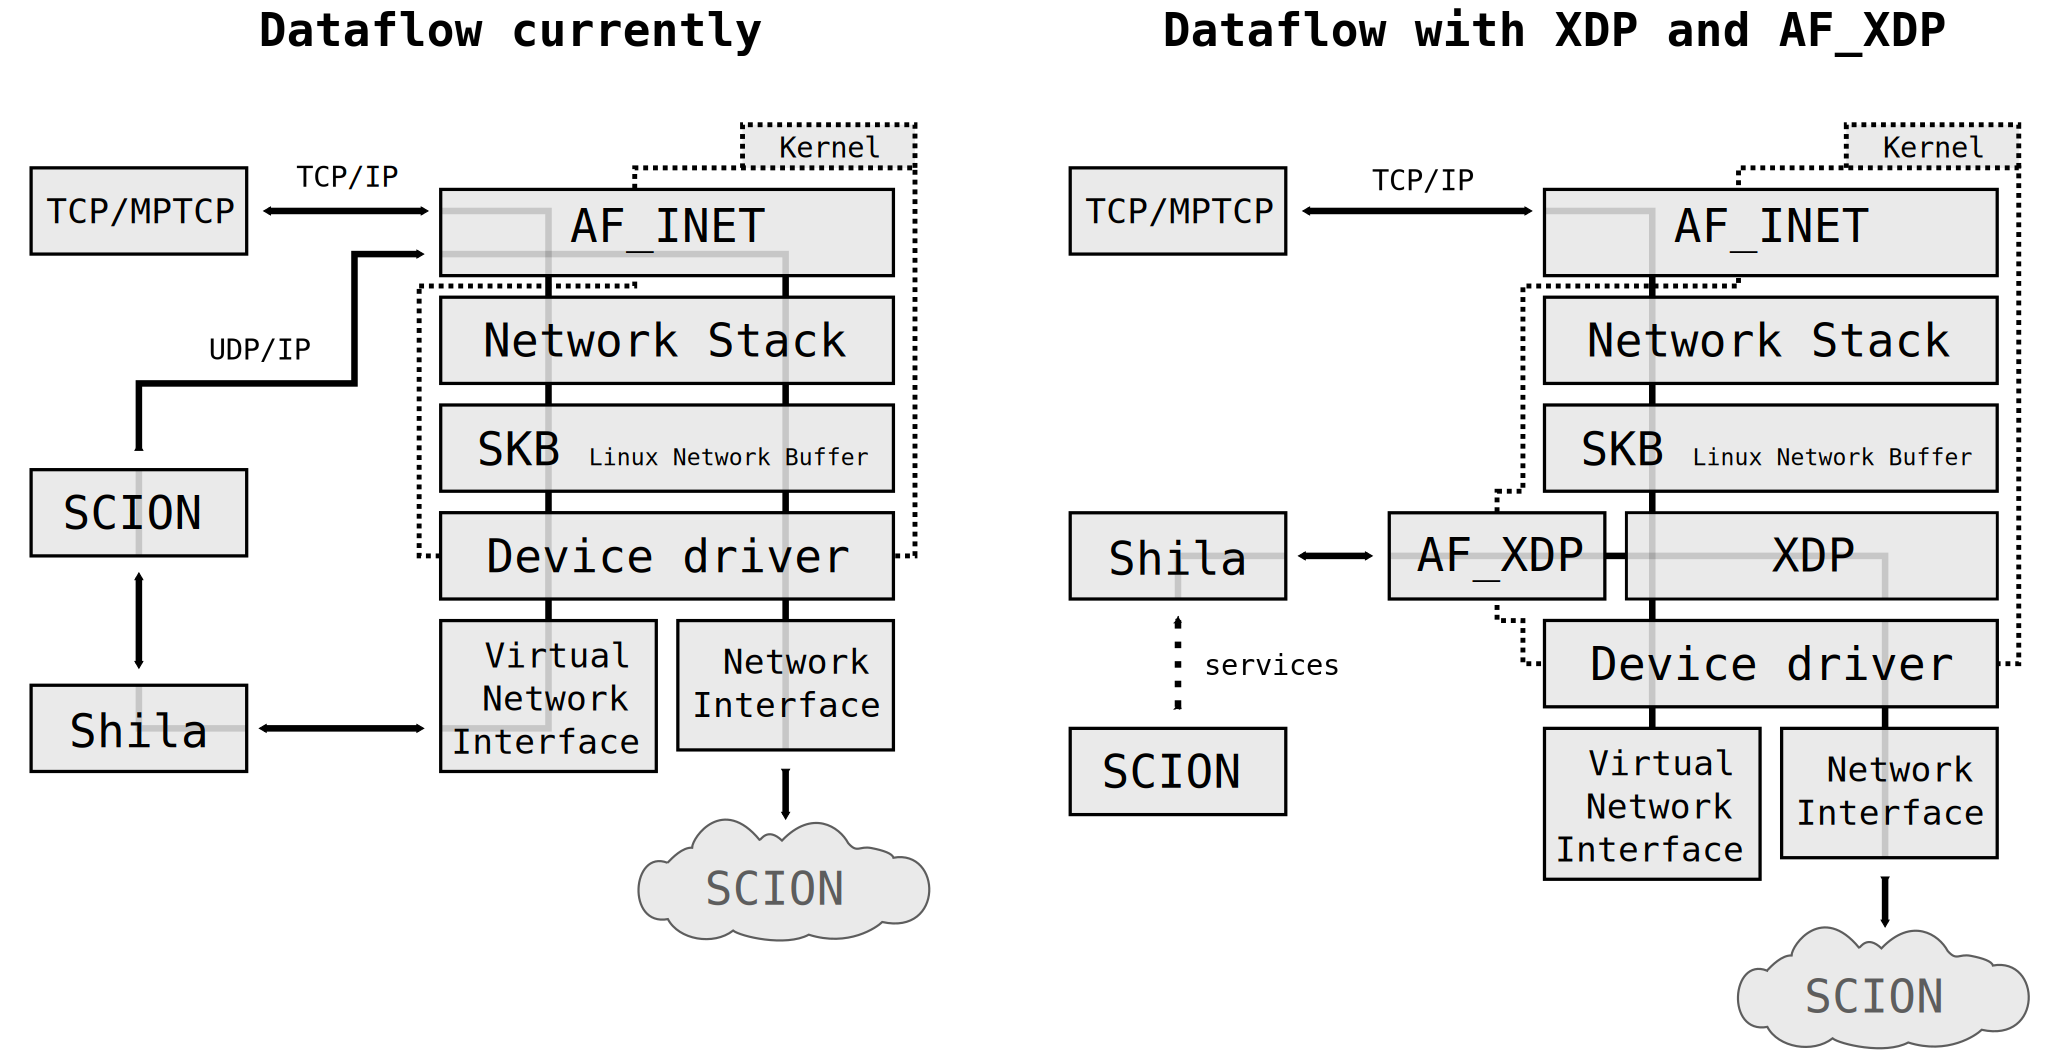
\includegraphics[scale=0.2]{../illustrations/futureWork/DetourAndWithXDP.pdf}   
		\caption[Caption for the list of figures.]{On the left side, the path taken by data exchanged via MPTCP over SCION is illustrated. In both endpoints, the kernel is traversed twice. The right side illustrates the path taken when using XDP (eXpress Data Path). This time the kernel is only traversed once per endpoint.}
		\label{fig:ShilaDetourKernel}
	\end{center}
\end{figure}

XDP \cite{XDP,XDPGitHub}, short for eXpress Data Path, is a relatively recent approach to programmable packet processing. It is not the first technology that allows the programmable processing of packets, but its approach differs from known solutions.  Known products like the  DataPlane Development Kit (DPDK) \cite{DPDK} bypass the kernel at all. The complete control of the network hardware is hand over to the networking application residing in user space. This comes with the advantage that the costs caused by the userland-kernel boundary can be avoided. But the approach also has disadvantages. By completely bypassing the kernel, useful functionalities of the network stack are not available, which complicates the implementation using these so-called kernel bypass approaches. Besides, are important security and isolation mechanisms of the kernel, ensuring the stability and security of the system, circumvented as well. 

In contrast, with XDP, programmable packet processing is integrated directly into the kernel. Even before the kernel handles an incoming packet, the so-called XDP driver hook is executed as part of the device driver. Within this customizable XDP program, there are various options for processing the packet. These include parsing, editing of header or payload or even the creation of additional metadata. Once the hook is done, it has again multiple options: It can either drop the packet, directly send it out via the receiving interface or to hand it over to the networking stack. As a fourth option, the packet can be redirected to different destinations, one of them is called AF\_XDP. AF\_XDP \cite{AFXDPPaper, AFXDPWeb,AFXDPWeb2} is a special socket type that allows the exchange of raw packets between the network interface and a userland application at a high speed. In addition to AF\_XDP, the XDP driver hook can use another process or network interface as further destinations for forwarding the packet.

With the help of XDP and AF\_XDP, the double way through the kernel can be saved. The shortened path of the data is illustrated in Figure \ref{fig:ShilaDetourKernel} on the right.  Packets sent from the TCP/MPTCP instance towards the virtual interface can be redirected to Shila using a corresponding XDP hook\footnote{XDP provides mechanisms to redirect outgoing traffic as well.}. Shila reads the IP datagrams from the AF\_XDP socket, extracts the necessary data and creates a SCION packet. This packet is then sent over the SCION network via the AF\_XDP socket of the outgoing network interface. On the receiving side, the same procedure is performed in reverse order. Shila unpacks the received SCION packet and creates the IP datagram which is then pushed through the network stack towards the receiving TCP/MPTCP instance.

Even if the proposed alternative is promising, the effort of implementation should not be underestimated. Since relatively new, the technology is constantly being revised and developed, occasional changes to the API must be expected. Furthermore requires XDP support from the network interface drivers to fully unfold its potential. Something which makes, at least at the moment, the usage of this technology less attractive. When approaching the implementation it should be taken into account that a part or maybe even the whole functionality of Shila, e.g. the parsing of the packets, can be integrated into an XDP. As already mentioned, the technology is constantly being developed and its functionality is being expanded. It is therefore desirable to investigate how far this integration is feasible, to maybe even save the way back into the userland.  
	
\section*{Namespace less solution}

\section*{Further measurements}

\section*{Avoidance of appnet}

\section*{Different criteria for the path selection}

